\chapter{TAXES}
\begin{chapquote}{Associates of Edwin L. Drake in 1859}
``Drill for oil? You mean drill into the ground to try and find oil? You're crazy.''
\end{chapquote}

\section{Personal taxes} \label{Personal taxes}

Figure \ref{fig:tax_rate_schedule} summarizes the US income tax rate schedule. As already said in section \ref{mortgages}, deductions are possible when paying interests, so it is possible that two people with the same income end up paying a different amount of taxes. 

\begin{figure}[h!]
\centering
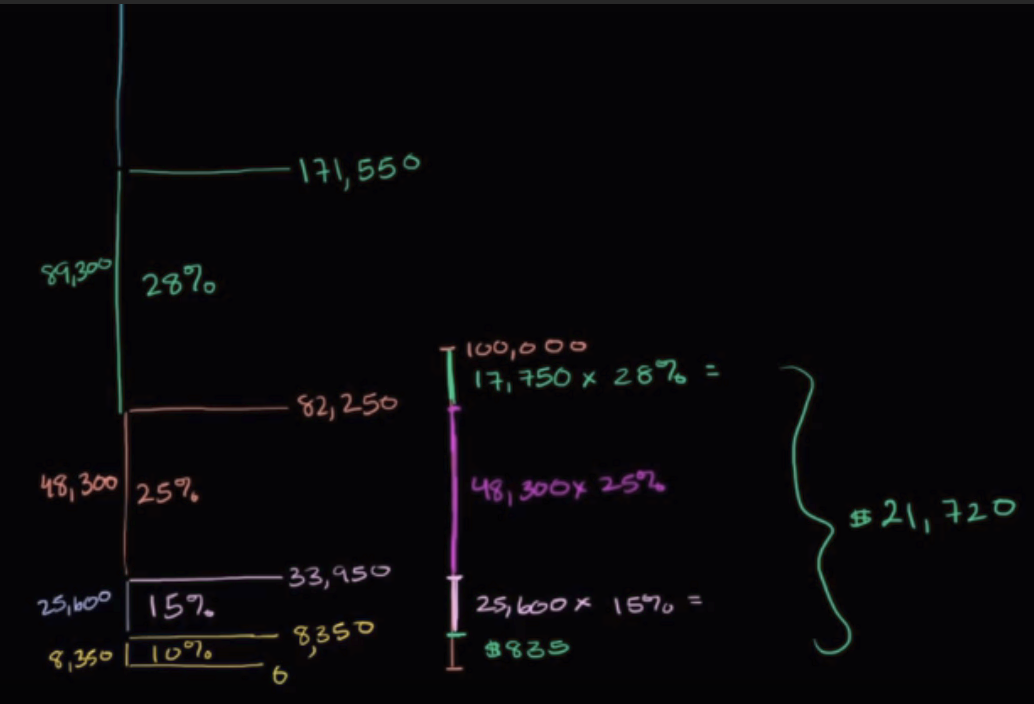
\includegraphics[width=0.8\textwidth]{images/tax_rate_schedule.png}
\caption{US income tax rate schedule.}
\label{fig:tax_rate_schedule}
\end{figure}

Sometimes it may happen that due to lots of deductions from an income, one can end up paying very low taxes and when they are less than a certain sum $AMT$, then this second sum is paid instead.  Alternative Minimum Tax (AMT) is a tax computed similarly to Figure \ref{fig:tax_rate_schedule} but with different tax rates and, as the name says, it is a minimum tax that every US citizen has to pay.

The estate tax, also known as inheritance tax, allows you to give all of your money, properties and so on, to someone when you pass away without any tax. If your estate is more than \$5 millions, say $S$, then you'll pay 35\% of taxes on the remaining part: $T = (S - \$5M) \cdot 0.35$. The reason behind this tax is that it exists only for very rich people and it's an incentive to make rich children start working or "a certain corrective against the development of a race of idle rich" as W. Churchill said in 1924. Also, this tax may look like a double-taxation system as we already pay taxes on our income, but in fact double taxation already happens everyday when we buy a product (VAT). 

In the US, there are taxes paid to the federal government and some states also add other state taxes. Different deductions are possible, depending on your status. If you're married you usually end up paying more taxes. This is known as marriage penalty, but this does not always occur. Some examples are reported in Figure \ref{fig:marriage_penalty}. 

\begin{figure}[h!]
\centering
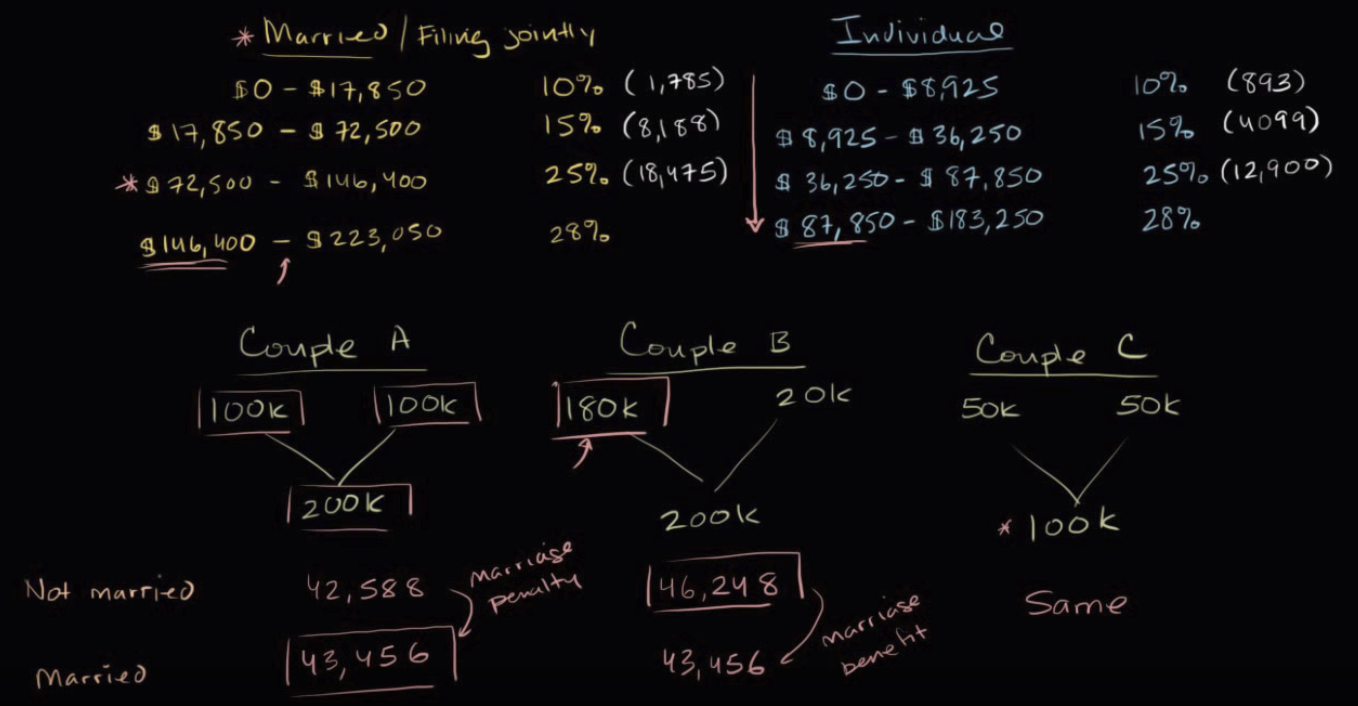
\includegraphics[width=0.8\textwidth]{images/marriage_penalty.png}
\caption{Different examples of marriage taxation.}
\label{fig:marriage_penalty}
\end{figure}

If paying taxes as married and filing jointly does not mean lower taxes as in the first example, you may think to pay separately, but that's not an option. You'd fall under the "filing separately" option where you end up paying the same amount of taxes as can be seen in Figure \ref{fig:marriage_separately} 

\begin{figure}[h!]
\centering
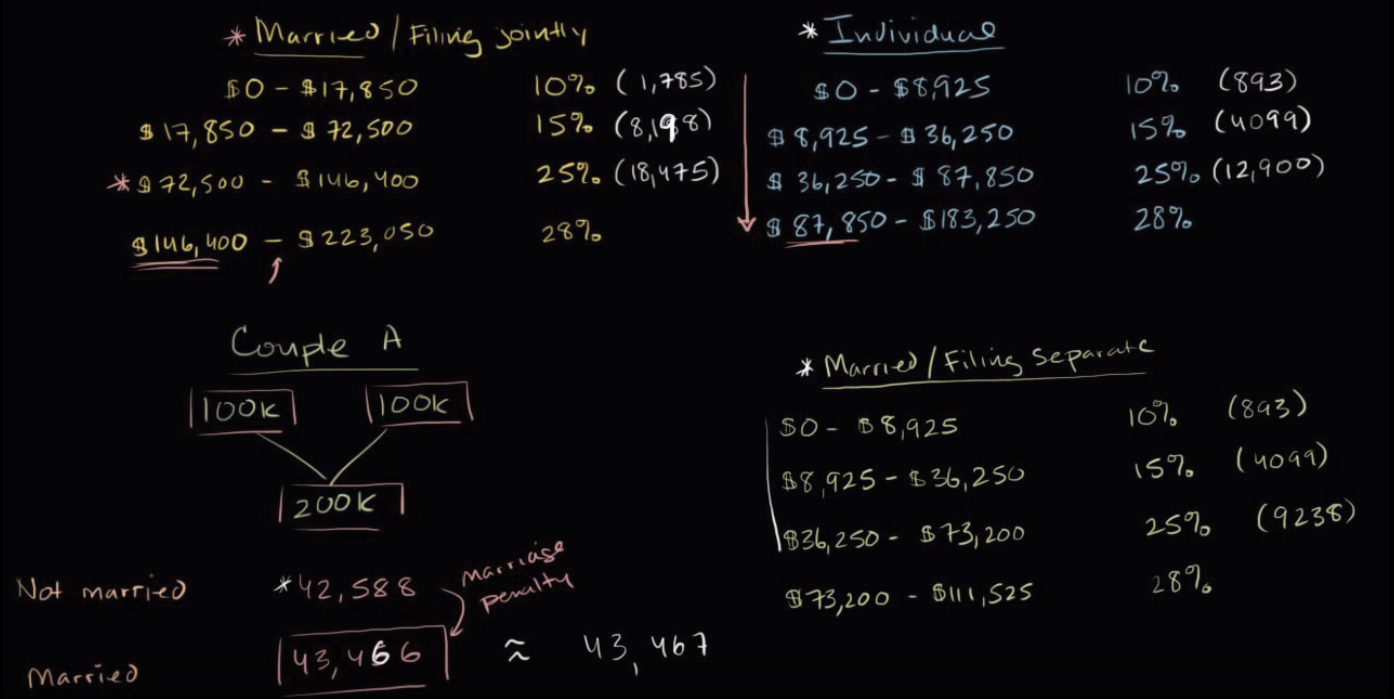
\includegraphics[width=0.8\textwidth]{images/marriage_separately.png}
\caption{Married, filing separately.}
\label{fig:marriage_separately}
\end{figure}

\section{Corporate taxation}

A corporation is a legal entity that can "act" like a person. It has limited liability and its ownership can be shared. The corporation has a certain amount of capital coming from the founders (or owners and investors), but if something bad happens, like an accident or a natural disaster, then the corporation can go bankrupt and all the money of the company is gone, but the owners do not lose their own private assets unrelated to the corporation. Being protected from this kind of events encourage entrepreneurship and starting a business, but it also levels all the possible entrepreneurs, in that a rich businessman with lots of assets and a simple middle-class person can both decide to start a corporation with an initial capital $C$, without being afraid of losing other money. The counterargument to this is that when the corporation goes bankrupt there will be someone else losing money. This is a trade-off in modern society.

There exists different types of corporations. The biggest one is a C-corp, such as big public companies. They will have a double-taxation system where the company pays taxes, but also the shareholders pay taxes on their profit. Other smaller corporations include: LLC, LP, LLP, S-corp. They have a single taxation. 

Some companies may also create a subsidiary in another countries with lower taxes and report the bigger part of their gross profit coming from the other countries ending up paying considerably less taxes. Nevertheless, if a company claims to have a large amount of money coming from abroad (where it pays less taxes) they have to send it back to the initial country (with higher taxes) somehow. In this last step, usually, there is a tax to prevent this kind of illicit transactions.

\section{Additional notes}

\subsection{Tax selling}
Imagine you have just sold stocks from company A and you made a profit of \$1k and this is all your profit for this year. If you had to pay taxes on this profit with a rate of 20\%, you'd pay \$200. Assume that you also have 100 stocks from company B that you bought for \$10 each and they are now trading at \$5, with stable or non-increasing trend. So, before the tax season, you decide to sell stocks B and lose \$500. Now your profit is \%500 and your taxes are \$100. Hence, the purpose of tax selling is to sell assets that are in a loss position for you without a positive trend in the near future and reduce your taxable income.

It is important to note that the IRS is aware that the deductibility of investment losses might tempt investors to sell at a loss, deduct the loss, and then turn around and buy the same stock again in an effort to evade taxes. This practice is called a wash sale, and the IRS has wash sale rules in place to prevent investors from selling and buying back stocks to avoid paying taxes.
